\documentclass[12pt]{article}

\usepackage[margin=1in]{geometry}
\usepackage{amsmath,amsthm,amssymb}
\usepackage{mathrsfs}
\usepackage{mathtools}
\usepackage{enumitem}
\usepackage{physics}

\usepackage{tikz}
\usetikzlibrary{calc,decorations.markings}

\newcommand{\magsq}[1]{\big|#1\big|^2}
\newcommand{\avg}[1]{\left<#1\right>}
\newcommand{\fullint}{\int_{-\infty}^\infty}
\newcommand{\fullintd}[1]{\fullint\dd#1\:}
\newcommand{\cint}[2]{\int_{#1}^{#2}}
\newcommand{\cintd}[3]{\cint{#1}{#2}\dd#3\:}
\newcommand\treq{\stackrel{\mathclap{\tiny\mbox{Tr}}}{=}}

\begin{document}
	
\title{Exercise Set 7}
\author{Sean Ericson \\ Phys 633}
\maketitle

\section*{Monday}
\subsection*{Exercise 1}
\begin{center}
    \resizebox{250pt}{!}{
        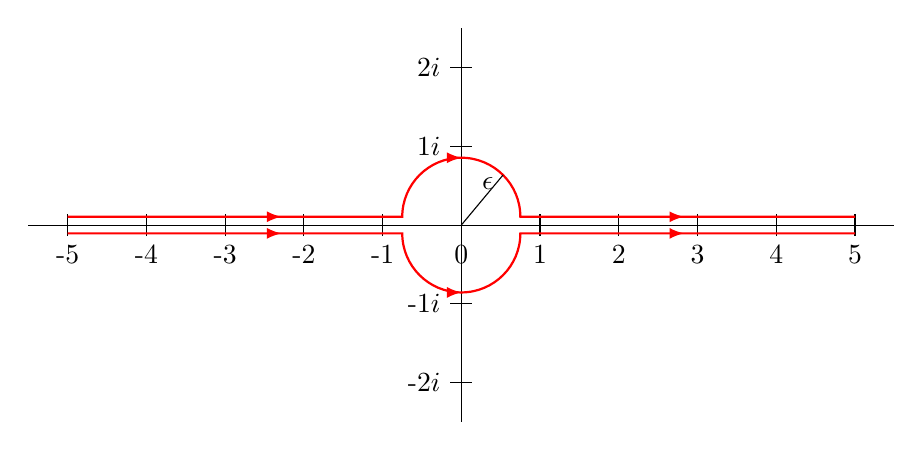
\begin{tikzpicture}
            \draw (0,-2.5) -- (0,2.5);  % Axis
            \draw (-5.5,0) -- (5.5,0);   
            \foreach \y in {-5,...,5} {
            \draw (\y,-4pt) -- (\y,4pt) node[pos=0,below] {\y};
            }
            \foreach \y in {-2,-1,1,2}{
                \draw (-4pt,\y) -- (4pt,\y) node[pos=0,left] {\y $i$};
            }
            
            \def\r{0.75}
            \pgfmathsetmacro\s{\r/sqrt(2)}
            \draw[thick,red,yshift=3pt,
            decoration={ markings,  % This schema allows for fine-tuning the positions of arrows
            mark=at position 0.25 with {\arrow{latex}},
            mark=at position 0.5 with {\arrow{latex}},
            mark=at position 0.8 with {\arrow{latex}}}, 
            postaction={decorate}]
            (-5,0) -- (-\r,0) arc (180:0:\r) -- (\r,0) -- (5,0);
        
            \draw[thick,red,yshift=-3pt,
            decoration={ markings,  % This schema allows for fine-tuning the positions of arrows
            mark=at position 0.25 with {\arrow{latex}},
            mark=at position 0.5 with {\arrow{latex}},
            mark=at position 0.8 with {\arrow{latex}}}, 
            postaction={decorate}]
            (-5,0) -- (-\r,0) arc (-180:0:\r) -- (\r,0) -- (5,0);

            \coordinate (A) at (0,0);
            \coordinate (B) at (\s,\s);
            \draw (A) -- ([yshift=3pt]B);

            \node[below,left] at (B) {$\epsilon$};

        \end{tikzpicture}
    }
\end{center}
For any function $f(z)$ that is analytic throught an $\epsilon$-disk centered on the origin, as $\epsilon\to 0$ we can approximate the value of $f$ for points on the circular portions of the above contour integrals by its value at the origin $f(0)$. In the case of an integrand of the form $f(z)/z$, the circular portion on the upper integral gives
\[ -f(0)\cint{\pi}{0}\frac{1}{\epsilon e^{i\theta}}\epsilon \dd\theta = f(0)\cint{0}{\pi}e^{-i\theta}\dd\theta = -2if(0), \]
while the circular portion on the lower integral gives
\[ f(0)\cint{\pi}{2\pi}\frac{1}{\epsilon e^{i\theta}}\epsilon \dd\theta = f(0)\cint{\pi}{2\pi}e^{-i\theta}\dd\theta = 2if(0), \]
The circular portions of both integrals therfore cancel, and we're left with just two integrals over the real line that skip the origin, verifying the equivalence of the two definitions. 

\section*{Tuesday}
Echoes and meeps!

\end{document}